\documentclass[paper=a4, fontsize=11pt]{scrartcl} % A4 paper and 11pt font size

\usepackage{float}
\usepackage{graphicx}
\usepackage[T1]{fontenc} % Use 8-bit encoding that has 256 glyphs
%\usepackage{fourier} % Use the Adobe Utopia font for the document - comment this line to return to the LaTeX default
\usepackage[english]{babel} % English language/hyphenation
\usepackage{amsmath,amsfonts,amsthm} % Math packages

\usepackage{lipsum} % Used for inserting dummy 'Lorem ipsum' text into the template

\usepackage{sectsty} % Allows customizing section commands
\allsectionsfont{\centering \normalfont\scshape} % Make all sections centered, the default font and small caps

\usepackage{fancyhdr} % Custom headers and footers
\pagestyle{fancyplain} % Makes all pages in the document conform to the custom headers and footers
\fancyhead{} % No page header - if you want one, create it in the same way as the footers below
\fancyfoot[L]{} % Empty left footer
\fancyfoot[C]{} % Empty center footer
\fancyfoot[R]{\thepage} % Page numbering for right footer
\renewcommand{\headrulewidth}{0pt} % Remove header underlines
\renewcommand{\footrulewidth}{0pt} % Remove footer underlines
\setlength{\headheight}{13.6pt} % Customize the height of the header

\numberwithin{equation}{section} % Number equations within sections (i.e. 1_1, 1_2, 2_1, 2_2 instead of 1, 2, 3, 4)
\numberwithin{figure}{section} % Number figures within sections (i.e. 1_1, 1_2, 2_1, 2_2 instead of 1, 2, 3, 4)
\numberwithin{table}{section} % Number tables within sections (i.e. 1_1, 1_2, 2_1, 2_2 instead of 1, 2, 3, 4)

\setlength\parindent{0pt} % Removes all indentation from paragraphs - comment this line for an assignment with lots of text

%----------------------------------------------------------------------------------------
%	TITLE SECTION
%----------------------------------------------------------------------------------------

\newcommand{\horrule}[1]{\rule{\linewidth}{#1}} % Create horizontal rule command with 1 argument of height

\title{	
\normalfont \normalsize 
\horrule{0.5pt} \\[0.4cm] % Thin top horizontal rule
\huge Assignment1 \\ % The assignment title
\horrule{2pt} \\[0.5cm] % Thick bottom horizontal rule
}

\author{Qinyun Song 5120309059} % Your name

\date{\normalsize\today} % Today's date or a custom date

\begin{document}

\maketitle % Print the title

%----------------------------------------------------------------------------------------
%	PROBLEM 1
%----------------------------------------------------------------------------------------
\newpage
\section{Convert the NFAs to DFAs}
\subsection{Figure 3.26}
\subsubsection*{Transition Table}
\begin{table}[H]
\centering
\begin{tabular}{|c|c|c|c|}
\hline
NFA State & DFA State & a & b \\
\hline
\{0, 1, 3\} & A & B & C \\
\hline
\{2\} & B & B & $\emptyset$ \\
\hline
\{4\} & C & $\emptyset$ & C \\
\hline
\end{tabular}
\end{table}
\subsubsection*{DFA}
\begin{figure}[H]
\centering
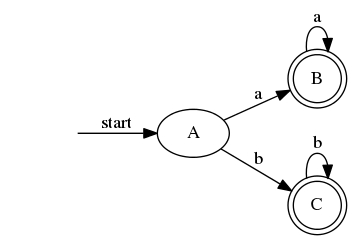
\includegraphics[width=0.5\textwidth]{1_1.png}
%\caption{DFA for Fig. 3.26}
\label{fig:1_1}
\end{figure}

\subsection{Figure 3.29}
\subsubsection*{Transition Table}
\begin{table}[H]
\centering
\begin{tabular}{|c|c|c|c|}
\hline
NFA State & DFA State & a & b \\
\hline
\{0\} & A & B & A \\
\hline
\{0, 1\} & B & C & B \\
\hline
\{0, 1, 2\} & C & C & D \\
\hline
\{0, 1, 2, 3\} & D & C & D \\
\hline
\end{tabular}
%\caption{Transition Table for Fig. 3.29}
\end{table}
\subsubsection*{DFA}
\begin{figure}[H]
\centering
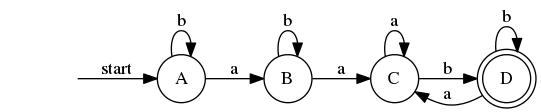
\includegraphics[width=0.8\textwidth]{1_2.png}
%\caption{DFA for Fig. 3.29}
\label{fig:1_2}
\end{figure}

\subsection{Figure 3.30}
\subsubsection*{Transition Table}
\begin{table}[H]
\centering
\begin{tabular}{|c|c|c|c|}
\hline
NFA State & DFA State & a & b \\
\hline
\{0, 1, 2, 3\} & A & A & A \\
\hline
\end{tabular}
\end{table}
\subsubsection*{DFA}
\begin{figure}[H]
\centering
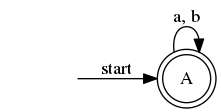
\includegraphics[width=0.35\textwidth]{1_3.png}
%\caption{DFA for Fig. 3.30}
\label{fig:1_3}
\end{figure}

%----------------------------------------------------------------------------------------
%	PROBLEM 2
%----------------------------------------------------------------------------------------
\newpage
\section{Use Algorithm 3.22 to Simulate the NFAs on Input "aabb"}
\subsection*{Figure 3.29}
\begin{figure}[H]
\centering
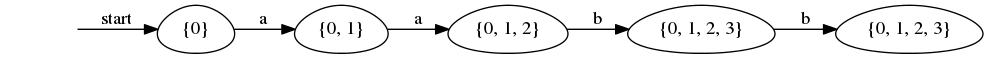
\includegraphics[width=1.1\textwidth]{2_1.png}
%\caption{Simulation for Fig. 3.29}
\label{fig:2_1}
\end{figure}

\subsection*{Figure 3.30}
\begin{figure}[H]
\centering
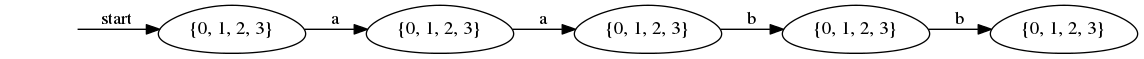
\includegraphics[width=1.1\textwidth]{2_2.png}
%\caption{Simulation for Fig. 3.30}
\label{fig:2_2}
\end{figure}

%----------------------------------------------------------------------------------------

%----------------------------------------------------------------------------------------
%	PROBLEM 3
%----------------------------------------------------------------------------------------
\newpage
\section{Convert the Regular Expressions to DFA}
\subsection{(a | b)*}
\subsubsection*{NFA}
\begin{figure}[H]
\centering
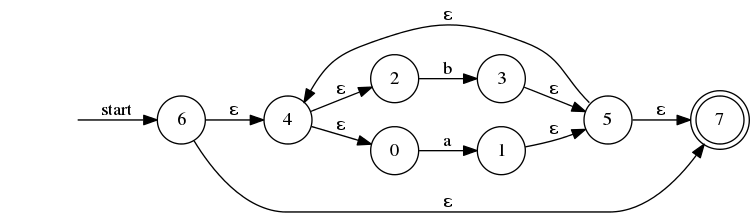
\includegraphics[width=0.8\textwidth]{3_1_1.png}
%\caption{NFA of 3.1}
\label{fig:3_1_1}
\end{figure}
\subsubsection*{Transition Table}
\begin{table}[H]
\centering
\begin{tabular}{|c|c|c|c|}
\hline
NFA State & DFA State & a & b \\
\hline
\{0, 2, 4, 6, 7\} & A & B & C \\
\hline
\{0, 1, 2, 4, 5, 7\} & B & B & C \\
\hline
\{0, 2, 3, 4, 5, 7\} & C & B & C \\
\hline
\end{tabular}
\end{table}
\subsubsection*{DFA}
\begin{figure}[H]
\centering
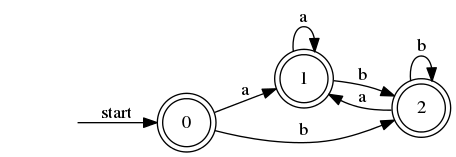
\includegraphics[width=0.65\textwidth]{3_1_2.png}
%\caption{DFA of 3.1}
\label{fig:3_1_2}
\end{figure}

\subsection{(a*|b*)*}
\subsubsection*{NFA}
\begin{figure}[H]
\centering
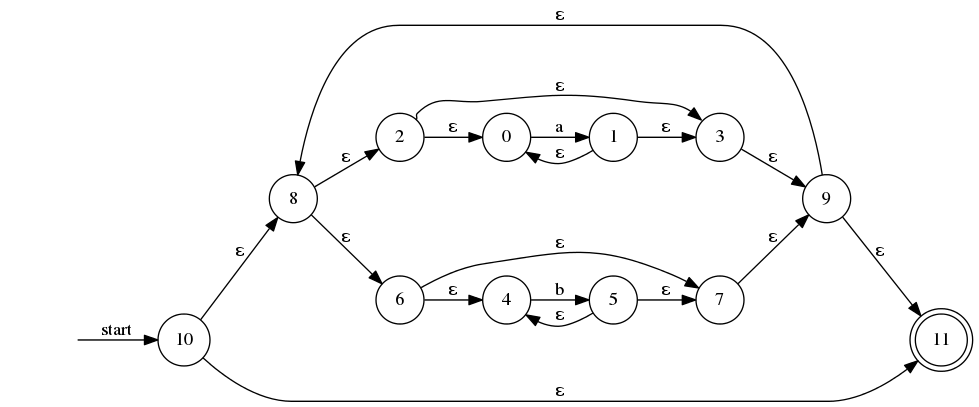
\includegraphics[width=1\textwidth]{3_2_1.png}
%\caption{NFA of 3.2}
\label{fig:3_2_1}
\end{figure}
\subsubsection*{Transition Table}
\begin{table}[H]
\centering
\begin{tabular}{|c|c|c|c|}
\hline
NFA State & DFA State & a & b \\
\hline
\{0, 2, 3, 4, 6, 7, 8, 9, 10, 11\} & A & B & C \\
\hline
\{0, 1, 2, 3, 4, 6, 7, 8, 9, 11\} & B & B & C \\
\hline
\{0, 2, 3, 4, 5, 6, 7, 8, 9, 11\} & C & B & C \\
\hline
\end{tabular}
\end{table}
\subsubsection*{DFA}
\begin{figure}[H]
\centering
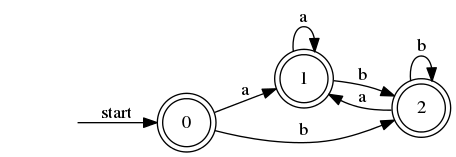
\includegraphics[width=0.6\textwidth]{3_2_2.png}
%\caption{DFA of 3.2}
\label{fig:3_2_2}
\end{figure}

\subsection{((ε|a)|b*)*}
\subsubsection*{NFA}
\begin{figure}[H]
\centering
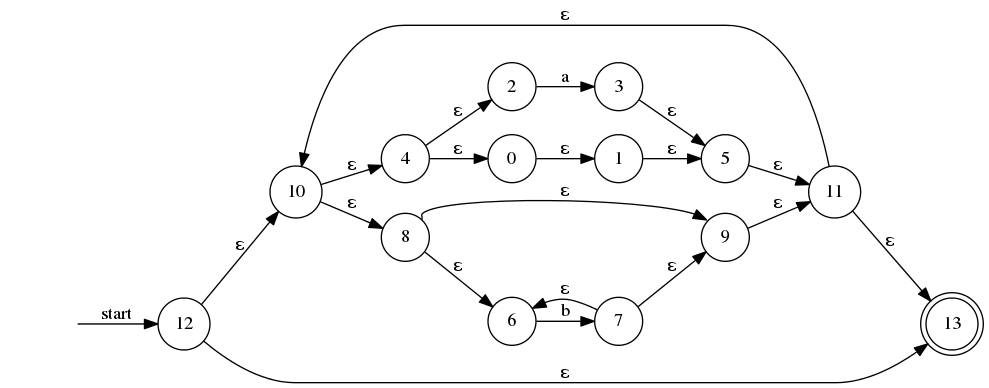
\includegraphics[width=1\textwidth]{3_3_1.png}
%\caption{NFA of 3.3}
\label{fig:3_3_1}
\end{figure}
\subsubsection*{Transition Table}
\begin{table}[H]
\centering
\begin{tabular}{|c|c|c|c|}
\hline
NFA State & DFA State & a & b \\
\hline
\{0, 1, 2, 4, 5, 6, 8, 9, 10, 11, 12, 13\} & A & B & C \\
\hline
\{0, 1, 2, 3, 4, 5, 6, 8, 9, 10, 11, 13\} & B & B & C \\
\hline
\{0, 1, 2, 4, 5, 6, 7, 8, 9, 10, 11, 13\} & C & B & C \\
\hline
\end{tabular}
\end{table}
\subsubsection*{DFA}
\begin{figure}[H]
\centering
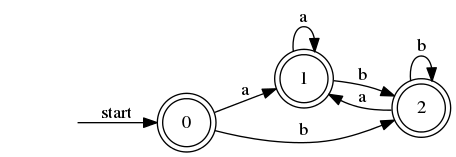
\includegraphics[width=0.6\textwidth]{3_3_2.png}
%\caption{DFA of 3.3}
\label{fig:3_3_2}
\end{figure}
%----------------------------------------------------------------------------------------

\end{document}
